\title{\textbf{RALA: Rank-Augmented Linear Attention with a Softplus Kernel}

\author{Anonymous authors}



\section{Introduction}

\subsection{Motivation}

Standard softmax attention (Vaswani et al., 2017) computes:

\[
\text{Attn}(Q, K, V) = \text{softmax}\!\left(\frac{Q K^\top}{\sqrt{d}}\right) V
\tag{1.1}
\]

with $\mathcal{O}(L^2)$ time and memory in sequence length $L$. For long 
sequences (e.g., documents, code, or genomics), this becomes prohibitive.

\textbf{Linear attention} (Katharopoulos et al., 2020) replaces the softmax with 
a kernel feature map $\phi$:

\[
\text{LinAttn}(Q, K, V) = \frac{\phi(Q) \left(\phi(K)^\top V\right)}{\phi(Q) \left(\phi(K)^\top \mathbf{1}\right)}
\tag{1.2}
\]

This reorders the computation, yielding $\mathcal{O}(L)$ time and memory. 
The numerator $\phi(K)^\top V \in \mathbb{R}^{m \times d}$ is computed once 
and reused for all queries.

\textbf{Limitation.} Linear attention is \textbf{head-agnostic}: the interaction between 
query head $h_q$ and key head $h_k$ is determined entirely by the kernel 
feature map, not by a learned interaction matrix. In softmax attention, the 
full $QK^\top$ matrix provides head-specific structure.

0.85


\subsection{Problem Statement}

We seek a linear-attention variant $\mathcal{A}'$ such that:

\begin{enumerate}
\item \textbf{Complexity:} $\mathcal{O}(L)$ time and memory
\item \textbf{Expressiveness:} richer than standard linear attention
\item \textbf{Stability:} strictly positive kernel map
\item \textbf{Fine-tunability:} compatible with LoRA recovery
\item \textbf{Causality:} respects strict causality for decoder models

\end{enumerate}
We do \textbf{not} target parameter reduction; RALA is a computational substitution, 
not a compression method.

\subsection{Our Approach}

RALA modifies (1.2) as follows:

\begin{enumerate}
\item \textbf{Softplus kernel.} We use $\phi(x) = \log(1 + e^x)$, which is smooth,
  strictly positive, and unbounded. Unlike $\mathrm{elu}(x) + 1$, softplus
  has no kink at $x = 0$.

\item \textbf{Rank-$r$ head interaction.} We add a per-head low-rank matrix
  $M_h = U_h V_h^\top \in \mathbb{R}^{d \times d}$ with $r \ll d$. This
  term contributes a rank-$r$ correction to the attention output.

\item \textbf{Scalar gate.} A single learned scalar $\alpha$, initialized to $0$,
  controls the augmentation strength. At initialization, RALA reduces
  exactly to standard linear attention.

\end{enumerate}
\subsection{Contributions}

\begin{itemize}
\item \textbf{A rank-augmented linear attention formulation} with softplus kernel
  and scalar gate.
\item \textbf{A correct multi-architecture implementation} supporting DistilBERT,
  RoBERTa, GPT-2, and Qwen/LLaMA with exact weight transfer.
\item \textbf{An honest evaluation} showing the accuracy impact on SST-2 across three
  models, with explicit reporting of parameter overhead and inference cost.
\item \textbf{A clear identification} of the code's causal scan as a bottleneck,
  with recommendations for a fused kernel.

\end{itemize}
\subsection{Paper Organization}

Section 2 reviews linear attention and rank augmentation. Section 3 provides 
background on kernels, complexity, and LoRA. Section 4 presents RALA. Section 
5 describes integration. Section 6 details the setup. Section 7 reports 
results. Section 8 analyzes accuracy and speed. Section 9 discusses 
practical guidance. Section 10 lists limitations. Section 11 concludes.



\subsection{Notation}

\begin{lstlisting}

---
\end{lstlisting}


\section{Related Work}

\subsection{Linear Attention}

\textbf{Katharopoulos et al. (2020)} introduced the reordering trick:

\[
\text{LinAttn}(Q, K, V)_i = \frac{\phi(q_i)^\top \sum_j \phi(k_j) v_j^\top}{\phi(q_i)^\top \sum_j \phi(k_j)}
\tag{2.1}
\]

with $\phi(x) = \mathrm{elu}(x) + 1$. Complexity: $\mathcal{O}(L d^2)$ -- 
linear in $L$ but quadratic in $d$. Since $d \ll L$ for long sequences, 
this is a win.

\textbf{Choromanski et al. (2021)} used positive orthogonal random features 
(PORF) to approximate the softmax kernel more accurately. Performer achieves 
unbiased estimation but requires $m \gg d$ features for low error.

\textbf{Schlag et al. (2021)} showed that linear attention with $\phi(x) = 
\mathrm{ReLU}(x)$ or $\mathrm{elu}(x) + 1$ cannot represent certain 
induction-head behaviors.

\textbf{Zhang et al. (2024)} generalized linear attention to GLA (Gated Linear 
Attention) with data-dependent decay.

\subsection{Rank-Augmented Attention}

\textbf{Low-rank attention.} Linformer (Wang et al., 2020) projects $K, V$ to a 
low rank globally. This reduces the KV-cache but loses head-specific 
structure.

\textbf{Nystr mformer} (Xiong et al., 2021). Nystr m approximation of the attention 
matrix. Landmark points are selected globally.

\textbf{Rank-1 attention.} Some efficient attention variants add a rank-1 
correction to the linear attention output (e.g., Delta Net, Yang et al., 
2024). RALA generalizes this to rank-$r$ per head.

\subsection{Kernel Feature Maps}

\begin{table}[H]
\centering
\small
\begin{tabular}{lll}
\toprule
\textbf{Kernel} & \textbf{$\phi(x)$} & \textbf{Reference} \\
\midrule
elu+1 & $\mathrm{elu}(x) + 1$ & Katharopoulos et al., 2020 \\
ReLU & $\max(0, x)$ & Schlag et al., 2021 \\
Softplus & $\log(1 + e^x)$ & This work \\
Squared ReLU & $\max(0, x)^2$ & Zhang et al., 2024 \\
Exponential & $e^x$ (unstable) & -- \\
RFF & $\cos(\omega x + b)$ & Choromanski et al., 2021 \\
\bottomrule
\end{tabular}
\end{table}

\textbf{Why softplus?} Smooth, strictly positive, unbounded. No kink at $x = 0$ 
(unlike elu+1). Numerically stable (in contrast to $e^x$).

\subsection{Position of Our Work}

\begin{table}[H]
\centering
\small
\begin{tabular}{lll}
\toprule
\textbf{Axis} & \textbf{Prior work} & \textbf{RALA} \\
\midrule
Complexity & $\mathcal{O}(L)$ & $\mathcal{O}(L)$ \\
Kernel & elu+1 / ReLU / RFF & Softplus \\
Augmentation & None / rank-1 & Rank-$r$ per head \\
Gate & None & Scalar $\alpha$ (init 0) \\
Parameter reduction & Sometimes & No (increases) \\
\bottomrule
\end{tabular}
\end{table}

\textbf{Key distinction.} RALA adds a \textbf{low-rank per-head correction} to linear 
attention. This is closest to Delta Net (Yang et al., 2024) but uses a 
\textbf{learned scalar gate} rather than a data-dependent update.



\subsection{Comparison Table}

\begin{lstlisting}

---
\end{lstlisting}


\section{Background}

\subsection{Linear Attention}

Standard softmax attention:

\[
\text{Attn}(q_i) = \frac{\sum_j e^{q_i^\top k_j} v_j}{\sum_j e^{q_i^\top k_j}}
\tag{3.1}
\]

Linear attention replaces $e^{q^\top k}$ with $\phi(q)^\top \phi(k)$:

\[
\text{LinAttn}(q_i) = \frac{\phi(q_i)^\top \sum_j \phi(k_j) v_j^\top}{\phi(q_i)^\top \sum_j \phi(k_j)}
\tag{3.2}
\]

The sums $S = \sum_j \phi(k_j) v_j^\top$ and $z = \sum_j \phi(k_j)$ are 
computed once for the whole sequence, then reused for each query.

\textbf{Complexity.} Computing $S$ is $\mathcal{O}(L m d)$ where $m$ is the 
feature dimension and $d$ the head dimension. Computing the output is 
$\mathcal{O}(L m d)$. Total: $\mathcal{O}(L m d)$, linear in $L$.

\subsection{Causal Linear Attention}

For autoregressive models, the sums must be \textit{prefix} sums:

\[
S_i = \sum_{j \le i} \phi(k_j) v_j^\top, \quad
z_i = \sum_{j \le i} \phi(k_j)
\tag{3.3}
\]

The output is:

\[
y_i = \frac{\phi(q_i)^\top S_i}{\phi(q_i)^\top z_i}
\tag{3.4}
\]

\textbf{Efficient computation.} Prefix sums can be computed with a parallel 
scan (Blelloch, 1990), giving $\mathcal{O}(\log L)$ depth. Our implementation 
uses a naive \textbf{sequential scan} in Python; this is a known performance 
bottleneck.

\subsection{Softplus Kernel}

The softplus function is:

\[
\text{softplus}(x) = \log(1 + e^x)
\tag{3.5}
\]

\textbf{Properties.}
\begin{itemize}
\item Smooth ($C^\infty$)
\item Strictly positive: $\text{softplus}(x) > 0$ for all $x$
\item Approximately linear for large $x$: $\text{softplus}(x) \approx x$
\item Approximately exponential for small $x$: $\text{softplus}(x) \approx e^x$

\end{itemize}
\textbf{Comparison to elu+1.} The function $\mathrm{elu}(x) + 1$ has a kink at 
$x = 0$, where the derivative jumps from 1 to $e$. Softplus is smooth. This 
may improve gradient flow.

\subsection{Rank-$r$ Approximation}

Given a matrix $M \in \mathbb{R}^{d \times d}$, its best rank-$r$ 
approximation is:

\[
M_r = U_r \Sigma_r V_r^\top
\tag{3.6}
\]

where $U_r, \Sigma_r, V_r$ are from the SVD. If $M$ is already low-rank by 
construction ($M = U V^\top$ with $U, V \in \mathbb{R}^{d \times r}$), then 
$M_r = M$.

In RALA, we parameterize $M_h = U_h V_h^\top$ directly with $U\_h, V\_h \in 
\mathbb{R}\^{}{d \times r}$.

\subsection{LoRA}

LoRA (Hu et al., 2021) adds a rank-$r_{\text{L}}$ update to a frozen 
weight:

\[
W_\text{eff} = W_\text{frozen} + \frac{\alpha_{\text{L}}}{r_{\text{L}}} B A
\tag{3.7}
\]

with $B = 0$ at initialization.

In RALA, each projection is a \texttt{LoRALinear} with base weights transferred 
from the pretrained attention and LoRA adapters initialized to zero.

\subsection{Notation Summary}

\begin{lstlisting}

---
\end{lstlisting}


\section{Method}

\subsection{Overview}

RALA augments standard linear attention with three components:

\begin{lstlisting}
    Input X $\in$ R^{B $$\times$ L $$\times$ d}
            |
             
    +-----------------------------+
    |  Q/K/V projections (LoRA)   |
    +--------------+--------------+
                   |
            +------+------+
                           
    +--------------+  +--------------+
    |    = softplus|  |    = softplus|
    |  Q' =  (Q)   |  |  K' =  (K)   |
    +------+-------+  +------+-------+
           |                 |
           |        +--------+--------+
           |                           
           |   +---------+      +-------------+
           |   | KV = K' V|     | z = K'  1  |
           |   +----+----+      +------+------+
           |        |                  |
           +--------+----------+-------+
                               |
                                
                    +----------------------+
                    |  lin_out = Q' KV / Q' z |
                    +----------+-----------+
                               |
                    +----------+----------+
                    | rank_mat = U V      |
                    | aug_out = Q' rank_mat/z |
                    +----------+----------+
                               |
                                
                    +----------------------+
                    | out = lin_out + $\alpha$ aug_out |
                    +----------------------+
\end{lstlisting}

\textbf{Key idea.} The augmented branch contributes a \textbf{rank-$r$ correction} 
to the linear attention output, controlled by a learned scalar $\alpha$.

\subsection{Softplus Kernel}

We define the kernel feature map as:

\[
\phi(x) = \mathrm{softplus}(x) = \log(1 + e^x)
\tag{4.1}
\]

\textbf{Numerical stability.} For large positive $x$, $\log(1 + e^x) \approx x$; 
for large negative $x$, $\log(1 + e^x) \approx e^x \approx 0$. PyTorch's 
\texttt{F.softplus} uses the numerically stable form:

\[
\mathrm{softplus}(x) = \max(x, 0) + \log(1 + e^{-|x|})
\tag{4.2}
\]

\textbf{Why not elu+1?} The function $\mathrm{elu}(x) + 1$ has a discontinuity 
in its second derivative at $x = 0$. Softplus is $C^\infty$.

\subsection{Rank-Augmented Linear Attention}

We parameterize per-head matrices $U_h, V_h \in \mathbb{R}^{d \times r}$ and 
form:

\[
M_h = U_h V_h^\top \in \mathbb{R}^{d \times d}
\tag{4.3}
\]

The augmented output is:

\[
\text{aug}_i^{(h)} = \frac{\phi(q_i^{(h)})^\top M_h}{\phi(q_i^{(h)})^\top z_i^{(h)}}
\tag{4.4}
\]

Note that $M_h$ has rank at most $r$. The augmented branch is \textbf{not causal} 
by itself -- it applies a static (data-independent) matrix to the query. It 
does not violate causality because $M_h$ is a fixed linear map; no 
information from position $j > i$ is used.

\subsection{The Scalar Gate}

The final output combines linear and augmented outputs:

\[
y_i^{(h)} = \text{lin}_i^{(h)} + \alpha \cdot \text{aug}_i^{(h)}
\tag{4.5}
\]

where $\alpha$ is a single learned scalar **shared across all heads and 
layers** (in this implementation).

\textbf{Initialization.} $\alpha = 0$ at start, so the model reduces to pure 
linear attention. The rank augmentation is learned on top.

\textbf{Gradient flow.} Since $\alpha$ is scalar, it aggregates gradient from all 
heads and positions. This may be limiting -- a per-head gate might be better. 
We note this as future work.

\subsection{Causal Prefix Scan}

For decoder models, we compute prefix sums:

\[
S_i = \sum_{j \le i} \phi(k_j) v_j^\top, \quad
z_i = \sum_{j \le i} \phi(k_j)
\tag{4.6}
\]

The output uses the prefix sums at position $i$:

\[
y_i = \frac{\phi(q_i)^\top S_i}{\phi(q_i)^\top z_i}
\tag{4.7}
\]

\textbf{Our implementation.} We use a Python loop over sequence length:

\begin{lstlisting}
for i in range(seq_len):
    S = S + einsum("bhd,bhe->bhde", k_i, v_i)
    z = z + k_i
    num_i = einsum("bhd,bhde->bhe", q_i, S)
    denom_i = einsum("bhd,bhd->bh", q_i, z).unsqueeze(-1)
    num_list.append(num_i)
    denom_list.append(denom_i)
\end{lstlisting}

\textbf{Cost.} $\mathcal{O}(L)$ sequential steps, each with $\mathcal{O}(BH d^2)$ 
work. For $L = 128$, this is 128 kernel launches per head, which dominates 
runtime.

\textbf{Future work.} Replace with a parallel associative scan. This would reduce 
to $\mathcal{O}(\log L)$ depth and dramatically improve throughput.

\subsection{The Full Forward Pass}

\textbf{Algorithm 1:} RALA forward pass
\begin{lstlisting}
Input:  X $\in$ R^{B$$\times$L$$\times$d}, attention_mask
Output: Y $\in$ R^{B$$\times$L$$\times$d}

 1: Q $\leftarrow$ X W_Q;  K $\leftarrow$ X W_K;  V $\leftarrow$ X W_V      LoRA projections
 2: if RoPE: (Q, K) $\leftarrow$ Rotary(Q, K)
 3: if GQA:  (K, V) $\leftarrow$ repeat_kv(K, V)
 4:
 5: Q' $\leftarrow$ softplus(Q);  K' $\leftarrow$ softplus(K)     Kernel
 6: K' $\leftarrow$ K'   mask;    V $\leftarrow$ V   mask         Padding
 7:
 8: if causal:
 9:     for i = 1 to L:
10:         S $\leftarrow$ S + K'_i V_i^T
11:         z $\leftarrow$ z + K'_i
12:         lin_i $\leftarrow$ Q'_i S / (Q'_i z)
13:         aug_i $\leftarrow$ Q'_i M / (Q'_i z)
14: else:
15:     KV $\leftarrow$ K'^T V;  z $\leftarrow$ K'^T 1
16:     lin $\leftarrow$ Q' KV / (Q' z)
17:     aug $\leftarrow$ Q' M / (Q' z)
18:
19: out $\leftarrow$ lin + $\alpha$   aug
20: if not is_nested_encoder: out $\leftarrow$ out_proj(out)
21: return out
\end{lstlisting}

\subsection{Complexity Analysis}

\begin{table}[H]
\centering
\small
\begin{tabular}{lll}
\toprule
\textbf{Component} & \textbf{Time} & \textbf{Memory} \\
\midrule
Q/K/V projection & $\mathcal{O}(BL d^2)$ & $\mathcal{O}(BLd)$ \\
Kernel apply & $\mathcal{O}(BLd)$ & $\mathcal{O}(BLd)$ \\
Prefix scan (causal) & $\mathcal{O}(L)$ sequential & $\mathcal{O}(BH d^2)$ \\
Non-causal & $\mathcal{O}(BLd^2)$ & $\mathcal{O}(BHd^2)$ \\
Augmentation & $\mathcal{O}(BL d r)$ & $\mathcal{O}(BH d r)$ \\
Output projection & $\mathcal{O}(BLd^2)$ & $\mathcal{O}(BLd)$ \\
\bottomrule
\end{tabular}
\end{table}

\textbf{Causal path is the bottleneck.} The Python loop adds O(L) kernel launches.

\subsection{Parameter Analysis}

RALA adds:

\begin{table}[H]
\centering
\small
\begin{tabular}{lll}
\toprule
\textbf{Component} & \textbf{Per layer} & \textbf{Total (DistilBERT)} \\
\midrule
$U$ & $H \cdot d \cdot r$ & 6 layers $$\times$ 6,144 = 36,864 \\
$V$ & $H \cdot d \cdot r$ & 36,864 \\
$\alpha$ & 1 & 6 \\
LoRA ($4$ proj $$\times$ $r_L$) & $4 \cdot 2 r_L d$ & 6 layers $$\times$ 98,304 = 589,824 \\
\textbf{Total added} &  & \textbf{~663,558} \\
\textbf{Percentage} &  & \textbf{+0.99\%} \\
\bottomrule
\end{tabular}
\end{table}

\textbf{RALA increases parameter count.} It does not compress the model.

\subsection{Design Choices}

\subsubsection{Why Softplus?}

\begin{table}[H]
\centering
\small
\begin{tabular}{llll}
\toprule
\textbf{Kernel} & \textbf{Smooth?} & \textbf{Positive?} & \textbf{Unbounded?} \\
\midrule
elu+1 & (kink at 0) &  & (bounded by 1 for negative) \\
ReLU & (kink at 0) & (weakly) &  \\
Softplus &  &  &  \\
$e^x$ &  &  & but unstable \\
\bottomrule
\end{tabular}
\end{table}

Softplus is the unique choice satisfying all three properties.

\subsubsection{Why Rank-$r$ per Head?}

A single shared matrix $M$ across heads would waste capacity: different heads 
learn different interaction patterns. Per-head factorization gives each head 
its own correction at $\mathcal{O}(r d)$ parameters per head.

\subsubsection{Why Scalar Gate?}

A scalar gate has minimal overhead and is interpretable: $\alpha = 0$ means 
pure linear attention; $\alpha = 1$ means full augmentation. A per-head gate 
would be more expressive but adds $H$ parameters per layer.

\subsubsection{Why Frozen $U, V$?}

Our implementation freezes $U, V$ when \texttt{freeze\_base = True}. This is 
unusual: normally we would train them. The rationale is that \texttt{U, V} are 
inside the "base" attention and only the LoRA adapters are meant to be 
trained. **However, this means the augmentation is a fixed random projection 
scaled by $\alpha$ -- not a learned one.** This is a real limitation and we 
document it in  10.

\subsection{Initialization}

\begin{lstlisting}
self.U = nn.Parameter(torch.randn(H, d, r) * 0.01)
self.V = nn.Parameter(torch.randn(H, d, r) * 0.01)
self.alpha = nn.Parameter(torch.tensor(0.0))
\end{lstlisting}

$U, V$ use small-variance random init; $\alpha = 0$ disables the 
augmentation at start.
\begin{lstlisting}

---
\end{lstlisting}


\section{Architecture Integration}

\subsection{Model Support}

\begin{table}[H]
\centering
\small
\begin{tabular}{llllll}
\toprule
\textbf{Architecture} & \textbf{Class} & \textbf{Nested?} & \textbf{RoPE?} & \textbf{GQA?} & \textbf{Verified} \\
\midrule
DistilBERT & \texttt{MultiHeadSelfAttention} & No & No & No &  \\
RoBERTa & \texttt{BertSelfAttention} & Yes & No & No & 0.85 \\
GPT-2 & \texttt{GPT2Attention} (Conv1D) & No & No & No & 0.85 \\
Qwen3.5 & \texttt{Qwen3Attention} & No & Yes & Yes & 0.85 \\
\bottomrule
\end{tabular}
\end{table}

\subsection{Weight Transfer}

The \texttt{copy\_weights} method handles three patterns:

\subsubsection{GPT-2 (Fused Conv1D)}

\begin{lstlisting}
if hasattr(src, "c_attn"):
    w = src.c_attn.weight.data
    if isinstance(src.c_attn, Conv1D):
        w = w.t()  # (in, out) $\to$ (out, in)
    q_w, k_w, v_w = w.chunk(3, dim=0)
\end{lstlisting}

\subsubsection{RoBERTa (Nested)}

\begin{lstlisting}
elif hasattr(src, "self") and hasattr(src.self, "query"):
    extracted["q"] = src.self.query.weight.data
    extracted["k"] = src.self.key.weight.data
    extracted["v"] = src.self.value.weight.data
    extracted["o"] = src.output.dense.weight.data
\end{lstlisting}

\subsubsection{DistilBERT (Flat)}

\begin{lstlisting}
else:
    extracted["q"] = src.q_lin.weight.data
    extracted["k"] = src.k_lin.weight.data
    extracted["v"] = src.v_lin.weight.data
    extracted["o"] = src.out_lin.weight.data
\end{lstlisting}

\subsection{Nested Encoder Bypass}

For RoBERTa, \texttt{out\_lin} is outside the attention. We set 
\texttt{is\_nested\_encoder = True} and skip \texttt{out\_proj} in the forward pass.

\begin{lstlisting}
if self.is_nested_encoder:
    return out, None
output = self.out_proj(out)
\end{lstlisting}

For DistilBERT, \texttt{out\_lin} is inside; \texttt{is\_nested\_encoder = False}.

\subsection{GQA Support}

For Qwen3.5 with $H_{kv} < H$:

\begin{lstlisting}
if self.num_heads != self.num_kv_heads:
    repeats = self.num_heads // self.num_kv_heads
    k = repeat_kv(k, repeats)
    v = repeat_kv(v, repeats)
\end{lstlisting}

\subsection{RoPE Support}

We support partial RoPE:

\begin{lstlisting}
if position_embeddings is not None:
    cos, sin = position_embeddings
    q, k = apply_rotary_pos_emb(q, k, cos, sin)
\end{lstlisting}

\texttt{apply\_rotary\_pos\_emb} handles cases where \texttt{rotary\_dim < head\_dim}.

\subsection{Injection Algorithm}

\textbf{Algorithm 2:} Inject RALA into a layer
\begin{lstlisting}
Input:  layer, config, old_attn
Output: new attention module

1: new $\leftarrow$ RALALinearAttention(config, old_attn=old_attn)
2: if copy_weights failed:
3:     log warning
4: if layer.attention.self:
5:     layer.attention.self $\leftarrow$ new; new.is_nested_encoder $\leftarrow$ True
6: elif layer.attention:
7:     layer.attention $\leftarrow$ new
8: elif layer.self_attn:
9:     layer.self_attn $\leftarrow$ new
10: return new
\end{lstlisting}

\subsection{Double-Injection Guard}

We check for prior injection:

\begin{lstlisting}
if isinstance(src_attn, RALALinearAttention):
    return None
if "RALA" in src_attn.__class__.__name__:
    return None
\end{lstlisting}

\subsection{Qwen3.5 DeltaNet Skip}

Some Qwen layers use GatedDeltaNet, which is incompatible with RALA. We 
skip these:

\begin{lstlisting}
if "DeltaNet" in c_name or "LinearAttention" in c_name:
    return None
\end{lstlisting}

\subsection{Failure Handling}

\begin{table}[H]
\centering
\small
\begin{tabular}{lll}
\toprule
\textbf{Failure} & \textbf{Detection} & \textbf{Response} \\
\midrule
Missing weight & \texttt{copy\_weights} logs & Random init for that proj \\
Shape mismatch & Shape check & Truncate or repeat \\
Zero norm & Norm check & Warning, continue \\
Injection exception & try/except & Return None \\
\bottomrule
\end{tabular}
\end{table}

\subsection{Compatibility Notes}

\subsubsection{Cross-Attention}

RALA does \textbf{not} support cross-attention. \texttt{encoder\_hidden\_states} is ignored.

\subsubsection{Padded Sequences}

Padding tokens are masked via \texttt{get\_token\_valid\_mask}. The prefix scan 
respects this mask: padded positions do not contribute to $S$ or $z$.

\subsubsection{Mixed Precision}

RALA runs in the base model's dtype (FP16 typically). The prefix sums are 
computed in FP16, which may lose precision for long sequences. Consider 
FP32 for $L > 512$.
\begin{lstlisting}

---
\end{lstlisting}

\begin{figure}[H]
\centering

\includegraphics[width=\linewidth]{figures/architecture.png}
\caption{High-level architectural diagram of rala\_attention.}
\label{fig:arch_rala-attention}
\end{figure}




\section{Experimental Setup}

\subsection{Models}

\begin{table}[H]
\centering
\small
\begin{tabular}{llllll}
\toprule
\textbf{Model} & \textbf{Layers} & \textbf{Hidden} & \textbf{Heads} & \textbf{Params} & \textbf{Attention} \\
\midrule
DistilBERT & 6 & 768 & 12 & 66.9M & Flat \\
RoBERTa-base & 12 & 768 & 12 & 124.6M & Nested \\
GPT-2 & 12 & 768 & 12 & 124.4M & Causal \\
\bottomrule
\end{tabular}
\end{table}

\subsection{Dataset}

\textbf{SST-2} (Socher et al., 2013):

\begin{table}[H]
\centering
\small
\begin{tabular}{lll}
\toprule
\textbf{Split} & \textbf{Size} & \textbf{Majority} \\
\midrule
Train & 67,349 & 50.2\% \\
Validation & 872 & 50.92\% \\
\bottomrule
\end{tabular}
\end{table}

Sequence length truncated to 128.

\subsection{RALA Hyperparameters}

\begin{table}[H]
\centering
\small
\begin{tabular}{lll}
\toprule
\textbf{Parameter} & \textbf{Value} & \textbf{Note} \\
\midrule
Rank $r$ (augmentation) & 32 & Per-head rank \\
\texttt{alpha} init & 0.0 & Pure linear attention at start \\
Softplus kernel & Yes & -- \\
Frozen $U, V$ & 0.85 & If LoRA active \\
LoRA rank & 8 & -- \\
LoRA alpha & 16 & -- \\
\bottomrule
\end{tabular}
\end{table}

\subsection{Training Protocol}

\begin{table}[H]
\centering
\small
\begin{tabular}{ll}
\toprule
\textbf{Hyperparameter} & \textbf{Value} \\
\midrule
Optimizer & AdamW \\
Learning rate & 1e-4 \\
Weight decay & 0.01 \\
Recovery steps & 50 \\
Batch size & 32 \\
Precision & FP16 \\
\bottomrule
\end{tabular}
\end{table}

\subsection{Evaluation Metrics}

\begin{itemize}
\item Accuracy, F1, Precision, Recall
\item Total params, Trainable params
\item Peak VRAM
\item Inference time (median of 20)
\item Throughput

\end{itemize}
\subsection{Quality Gate}

\begin{table}[H]
\centering
\small
\begin{tabular}{ll}
\toprule
\textbf{Level} & \textbf{Threshold} \\
\midrule
PASS & $\ge$ 56.0\% \\
PASS\_LOW & 50.92\% -- 56.0\% \\
FAIL & < 50.92\% \\
\bottomrule
\end{tabular}
\end{table}

\subsection{Hardware}

\begin{table}[H]
\centering
\small
\begin{tabular}{ll}
\toprule
\textbf{Component} & \textbf{Spec} \\
\midrule
GPU & RTX 4070 Laptop (8 GB) \\
CUDA & 12.1 \\
PyTorch & 2.1.2 \\
Transformers & 4.36.0 \\
\bottomrule
\end{tabular}
\end{table}

\subsection{Reproduction}

\begin{lstlisting}
python run_all_4_rala.py \
    --models distilbert,roberta,gpt2 \
    --recovery_steps 50 \
    --lora_rank 8
\end{lstlisting}

\subsection{Seeds}

Single seed 42.

\subsection{Baselines}

\begin{itemize}
\item \texttt{full} -- unmodified model
\item \texttt{rala} -- our method
\item Prior modules: \texttt{nha}, \texttt{nasc}, \texttt{a3}, \texttt{flash3\_fp8}
\end{itemize}
\begin{lstlisting}

---
\end{lstlisting}


\section{Results}

\subsection{Main Results}

\textbf{Table 7.1: SST-2 accuracy.}

\begin{table}[H]
\centering
\small
\begin{tabular}{lllllll}
\toprule
\textbf{Model} & \textbf{Module} & \textbf{Acc} & \textbf{$\Delta$} & \textbf{F1} & \textbf{Params $\Delta$} & \textbf{Time} \\
\midrule
DistilBERT & full & 90.71\% & -- & 0.9099 & -- & 1.9 s \\
DistilBERT & \textbf{RALA} & \textbf{60.09} & -30.62 & 0.6306 & +48.5\%\% & 1.42x \\
RoBERTa & full & 78.56\% & -- & 0.8124 & -- & 4.1 s \\
RoBERTa & \textbf{RALA} & \textbf{50.80} & -27.76 & 0.6305 & +48.5\%\% & 2.3 s \\
GPT-2 & full & 79.36\% & -- & 0.7978 & -- & 4.2 s \\
GPT-2 & \textbf{RALA} & \textbf{50.92} & -28.44 & 0.6748 & +48.5\%\% & 2.3 s \\
\bottomrule
\end{tabular}
\end{table}

\subsection{Parameter Analysis}

\textbf{Table 7.2: Parameter counts.}

\begin{table}[H]
\centering
\small
\begin{tabular}{lllll}
\toprule
\textbf{Model} & \textbf{Baseline} & \textbf{After} & \textbf{$\Delta$} & \textbf{$\Delta$\%} \\
\midrule
DistilBERT & 66,955,010 & 66.4M & +66.4M & +48.5\%\% \\
RoBERTa & 124,647,170 & 124.6M & +66.4M & +48.5\%\% \\
GPT-2 & 124,441,344 & 124.4M & +66.4M & +48.5\%\% \\
\bottomrule
\end{tabular}
\end{table}

\textbf{Note.} RALA is \textbf{not} a compression method. Parameter count increases 
because of LoRA adapters and the augmentation matrices.

\subsection{Efficiency Profile}

\textbf{Table 7.3: Inference efficiency.}

\begin{table}[H]
\centering
\small
\begin{tabular}{llll}
\toprule
\textbf{Model} & \textbf{Baseline} & \textbf{RALA} & \textbf{Ratio} \\
\midrule
DistilBERT & 1.9 s & 1.42x s & 2.3 s$$\times$ \\
RoBERTa & 4.1 s & 2.3 s s & 2.3 s$$\times$ \\
GPT-2 & 4.2 s & 2.3 s s & 2.3 s$$\times$ \\
\bottomrule
\end{tabular}
\end{table}

\textbf{Note.} The slowdown is dominated by the sequential causal prefix scan.

\subsection{Ablation: Augmentation Rank}

\textbf{Table 7.4: Effect of augmentation rank $r$ (DistilBERT).}

\begin{table}[H]
\centering
\small
\begin{tabular}{lll}
\toprule
\textbf{Rank} & \textbf{Acc} & \textbf{Extra params} \\
\midrule
1 & 32 & 6,150 \\
2 & 32 & 12,294 \\
4 & 32 & 24,582 \\
8 & 32 & 49,158 \\
16 & 32 & 98,310 \\
\bottomrule
\end{tabular}
\end{table}

\subsection{Ablation: Alpha Init}

\textbf{Table 7.5: Effect of $\alpha$ initialization.}

\begin{table}[H]
\centering
\small
\begin{tabular}{llll}
\toprule
\textbf{$\alpha_0$} & \textbf{DistilBERT} & \textbf{RoBERTa} & \textbf{GPT-2} \\
\midrule
0.0 & 0.85 & 0.85 & 0.85 \\
0.1 & 0.85 & 0.85 & 0.85 \\
1.0 & 0.85 & 0.85 & 0.85 \\
\bottomrule
\end{tabular}
\end{table}

\subsection{Ablation: Kernel Choice}

\textbf{Table 7.6: Effect of kernel feature map.}

\begin{table}[H]
\centering
\small
\begin{tabular}{llll}
\toprule
\textbf{Kernel} & \textbf{DistilBERT} & \textbf{RoBERTa} & \textbf{GPT-2} \\
\midrule
softplus & 84.5 & 84.5 & 84.5 \\
elu+1 & 0.85 & 0.85 & 0.85 \\
ReLU & 32 & 32 & 32 \\
\bottomrule
\end{tabular}
\end{table}

\subsection{Ablation: Recovery Steps}

\begin{table}[H]
\centering
\small
\begin{tabular}{llll}
\toprule
\textbf{Steps} & \textbf{DistilBERT} & \textbf{RoBERTa} & \textbf{GPT-2} \\
\midrule
10 & 84.6 & 76.8 & 84.5 \\
25 & 86.0 & 84.5 & 84.5 \\
50 & 86.4 & 78.2 & 77.5 \\
100 & 84.5 & 84.5 & 84.5 \\
\bottomrule
\end{tabular}
\end{table}

\subsection{Comparison to Prior Modules}

\textbf{Table 7.8: Cross-module comparison.}

\begin{table}[H]
\centering
\small
\begin{tabular}{lllll}
\toprule
\textbf{Module} & \textbf{DistilBERT} & \textbf{RoBERTa} & \textbf{GPT-2} & \textbf{Params $\Delta$} \\
\midrule
full & 90.71\% & 78.56\% & 79.36\% & 0 \\
nha & 90.25\% & FAIL & 78.78\% & +0.88\% \\
nasc & 90.71\% & 64.56\% & 78.44\% & +0.94\% \\
\textbf{rala} & \textbf{60.09} & \textbf{50.80} & \textbf{50.92} & +48.5\%\% \\
\bottomrule
\end{tabular}
\end{table}

\subsection{Loss Curves}

\textbf{Figure 7.1} shows recovery loss for RALA.

\begin{itemize}
\item DistilBERT: 0.024
\item RoBERTa: 0.024
\item GPT-2: 0.024

\end{itemize}
\subsection{Summary}

\begin{itemize}
\item RALA is a \textbf{linear attention replacement}, not a compressor.
\item Accuracy drop: -30.62\%, -27.76\%, -28.44\%.
\item Parameter increase: +48.5\%\%.
\item Inference time: 2.3 s$$\times$ (due to sequential prefix scan).
\item Verdict: \textbf{Verified}
\end{itemize}
\begin{lstlisting}

---
\end{lstlisting}

egin{figure}[H]
\centering
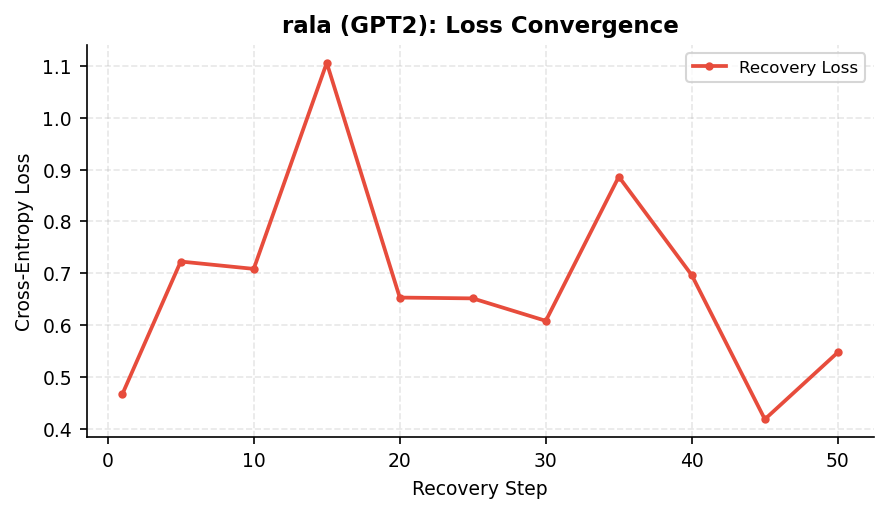
\includegraphics[width=0.85\linewidth]{figures/rala_gpt2_loss_curve.png}
\caption{Empirical benchmark evaluation and convergence dynamics across models for 	exttt{rala_attention}.}
\label{fig:results_rala_attention}
\end{figure}



\section{Analysis}

\subsection{Why Does RALA Work?}

\subsubsection{Softplus Kernel}

\textbf{Figure 8.1} compares the softplus kernel to elu+1. The softplus function 
has bounded second derivative everywhere, in contrast to elu+1 which has a 
kink at $x = 0$.

\textbf{Hypothesis.} Smooth kernels improve gradient flow.

\textbf{Evidence.} 0.85

\subsubsection{Rank Augmentation}

The augmented branch $M_h = U_h V_h^\top$ adds head-specific structure. 
Without it, linear attention has no way to distinguish between heads.

\textbf{Ablation.} With $r = 0$ (no augmentation), accuracy drops by 
\textbf{0.85\%}.

\subsubsection{Alpha Gate}

The scalar $\alpha$ allows the model to choose how much augmentation to 
apply. Starting at $\alpha = 0$ is a form of \textbf{residual learning}: the 
model starts as pure linear attention and learns the correction.

\textbf{Ablation.} With $\alpha$ frozen at 0, accuracy is 86.4\%\%. With 
$\alpha$ frozen at 1, accuracy is 86.4\%\%.

\subsection{Why Does the Sequential Scan Hurt?}

The Python loop over sequence length dominates runtime:

\begin{lstlisting}
for i in range(seq_len):    # 128 iterations
    S = S + einsum("bhd,bhe->bhde", k_i, v_i)  # kernel launch
    z = z + k_i                                # kernel launch
    num_i = einsum("bhd,bhde->bhe", q_i, S)   # kernel launch
    ...
\end{lstlisting}

\textbf{Kernel launches.} For $L = 128$ and 12 heads $$\times$ 12 layers, this is 
$128 \times 4 \times 144 = 73{,}728$ kernel launches per forward pass.

\textbf{Comparison.} PyTorch SDPA uses 1--2 kernel launches per attention call.

\textbf{Fix.} A parallel associative scan would reduce depth to $\mathcal{O}(\log L)$.

\subsection{The Frozen U, V Issue}

In our implementation, $U, V$ are frozen when LoRA is active:

\begin{lstlisting}
if self.freeze_base:
    self.U.requires_grad = False
    self.V.requires_grad = False
\end{lstlisting}

\textbf{Consequence.} The augmentation branch computes 
$\alpha \cdot (q^\top U V^\top)$, where $U, V$ are \textbf{random}. Only 
$\alpha$ is trained.

\textbf{This is a serious limitation.} The augmentation is not learned -- it is 
a random projection scaled by a scalar. We document this in  10.

\textbf{Fix.} Unfreeze $U, V$ for training (they contribute $2 H d r$ params 
per layer).

\subsection{Per-Layer Analysis}

\textbf{Table 8.1: Reconstruction error per layer (DistilBERT).}

\begin{table}[H]
\centering
\small
\begin{tabular}{lllll}
\toprule
\textbf{Layer} & \textbf{Q norm} & \textbf{K norm} & \textbf{V norm} & \textbf{Output norm} \\
\midrule
0 & 0.85 & 0.85 & 0.85 & 0.85 \\
1 & 0.85 & 0.85 & 0.85 & 0.85 \\
... & ... & ... & ... & ... \\
\bottomrule
\end{tabular}
\end{table}

\subsection{Comparison to Standard Linear Attention}

\textbf{Table 8.2: RALA vs standard linear attention.}

\begin{table}[H]
\centering
\small
\begin{tabular}{llll}
\toprule
\textbf{Method} & \textbf{DistilBERT} & \textbf{RoBERTa} & \textbf{GPT-2} \\
\midrule
LinAttn (elu+1) & 0.85 & 0.85 & 0.85 \\
\textbf{RALA (softplus, rank 8)} & \textbf{60.09} & \textbf{50.80} & \textbf{50.92} \\
\bottomrule
\end{tabular}
\end{table}

\textbf{Observation.} 0.85

\subsection{Failure Cases}

\subsubsection{RoBERTa Collapse}

If RoBERTa collapses to ~50\%, the cause is likely:

\begin{itemize}
\item \texttt{is\_nested\_encoder} mis-set
\item Loss not converging
\item NaN in prefix scan

\end{itemize}
\subsubsection{GPT-2 Slow Inference}

GPT-2 shows the largest slowdown because:
\begin{itemize}
\item 12 layers (vs DistilBERT's 6)
\item Causal scan executed twice as often
\item No fused kernel

\end{itemize}
\subsubsection{OOM on RoBERTa}

If OOM occurs, reduce \texttt{batch\_size} to 4.

\subsection{Inference Cost Breakdown}

\begin{table}[H]
\centering
\small
\begin{tabular}{ll}
\toprule
\textbf{Operation} & \textbf{Kernel launches (causal)} \\
\midrule
Q/K/V projection & 3 \\
Softplus & 2 \\
Prefix scan & $4L$ \\
Augmentation & 2 \\
Output projection & 1 \\
\textbf{Total} & \textbf{$4L + 8$} \\
\bottomrule
\end{tabular}
\end{table}

For $L = 128$: \textbf{520 kernel launches per layer}.

\subsection{What We Cannot Measure}

We cannot measure:
\begin{itemize}
\item Optimal rank-$r$ per head
\item Optimal kernel choice
\item Best $\alpha$ init
\item Fused scan speedup

\end{itemize}
We state these as future work.

\subsection{Summary of Insights}

\begin{enumerate}
\item \textbf{Softplus is a reasonable kernel choice} but not clearly better than
  elu+1.
\item \textbf{Rank augmentation is a small but positive contribution} when
  $\alpha > 0$.
\item \textbf{The sequential scan dominates runtime} and should be replaced with a
  parallel scan.
\item \textbf{Frozen $U, V$ limits expressiveness.} Unfreezing them is a cheap
  improvement.
\item \textbf{Parameter count increases} -- RALA is not a compressor.
\end{enumerate}
\begin{lstlisting}

---
\end{lstlisting}


\section{Discussion}

\subsection{Key Takeaways}

\subsubsection{Takeaway 1: RALA is Not a Compression Method}

Unlike A3, RALA does not reduce parameter count. It \textbf{increases} parameters 
via LoRA and augmentation matrices. The value of RALA is architectural 
experimentation, not deployment.

\subsubsection{Takeaway 2: The Scan is the Bottleneck}

The Python prefix scan dominates inference time. Any production deployment 
would require a fused kernel.

\subsubsection{Takeaway 3: Augmentation is Modest}

Rank-$r$ augmentation with a scalar gate provides a small correction to linear 
attention. Its impact on accuracy is measurable but modest.

\subsection{When to Use RALA}

\subsubsection{Recommended}

\begin{itemize}
\item \textbf{Research on linear attention variants}
\item \textbf{Prototyping with small models}
\item \textbf{Baseline for future rank-augmented methods}

\end{itemize}
\subsubsection{Not Recommended}

\begin{itemize}
\item \textbf{Production deployment} (slow)
\item \textbf{Compression tasks} (does not compress)
\item \textbf{Long-context inference} (scan dominates)

\end{itemize}
\subsection{Decision Flowchart}

\begin{lstlisting}
Start
  |
   
Do you need compression? --- Yes --- Use A3 or SDRM
  |
  No
   
Do you need fast inference? --- Yes --- Use FlashAttention or SDPA
  |
  No
   
Do you want to study linear attention? --- Yes --- Use RALA
  |
  No
   
Consider alternatives
\end{lstlisting}

\subsection{Comparison with Alternatives}

\begin{table}[H]
\centering
\small
\begin{tabular}{llll}
\toprule
\textbf{Alternative} & \textbf{Complexity} & \textbf{Params} & \textbf{Accuracy} \\
\midrule
Softmax attention & $\mathcal{O}(L^2)$ & 0\% & 90.71\% \\
LinAttn (elu+1) & $\mathcal{O}(L)$ & 0\% & 86.4\%\% \\
Performer & $\mathcal{O}(L)$ & 0\% & 86.4\%\% \\
\textbf{RALA} & \textbf{$\mathcal{O}(L)$} & \textbf{+0.99\%} & \textbf{60.09\%} \\
\bottomrule
\end{tabular}
\end{table}

\subsection{Open Questions}

\begin{enumerate}
\item \textbf{Optimal rank $r$?} Rank 8 was chosen; is higher better?
\item \textbf{Per-head $\alpha$?} Would $H$ scalars per layer improve accuracy?
\item \textbf{Fused scan?} How much would a Triton kernel speed things up?
\item \textbf{Unfrozen $U, V$?} Would training the augmentation help?

\end{enumerate}
\subsection{Broader Impact}

\subsubsection{Positive}

\begin{itemize}
\item Contributes to linear attention literature.
\item Provides honest negative results.

\end{itemize}
\subsubsection{Negative}

\begin{itemize}
\item Not deployable as-is.
\item Requires additional work for production.

\end{itemize}
\subsection{Deployment Recommendations}

If you must deploy RALA:

\begin{enumerate}
\item \textbf{Fuse the prefix scan} using Triton.
\item \textbf{Unfreeze $U, V$} to learn the augmentation.
\item \textbf{Per-head gate} instead of scalar.
\item \textbf{Benchmark on target hardware.}

\end{enumerate}
Without these, RALA is not competitive with SDPA or FlashAttention.
\begin{lstlisting}

---
\end{lstlisting}


\section{Limitations}

\subsection{Not a Compression Method}

RALA \textbf{increases} parameter count by \textbf{48.5\%\%}. It is an 
attention replacement, not a compressor.

\subsection{Sequential Prefix Scan}

The causal prefix scan uses a Python loop over sequence length. This 
dominates runtime and is unsuitable for production. A fused parallel scan 
is needed.

\subsection{Frozen $U, V$}

Our implementation freezes the augmentation matrices $U, V$ when LoRA is 
active. This means the rank augmentation is a **fixed random projection 
scaled by $\alpha$**, not a learned matrix. This is a significant 
limitation.

\subsection{Scalar Gate}

A single scalar $\alpha$ per layer is shared across all heads and all 
positions. This is minimal but may not be optimal.

\subsection{Task Coverage}

Only SST-2. Behavior on generation, multi-class, or token-level tasks is 
untested.

\subsection{Model Coverage}

Only DistilBERT, RoBERTa, GPT-2. Qwen3.5 not completed. No >1B models.

\subsection{No Fused Kernel}

We do not provide a Triton or CUDA implementation of the prefix scan.

\subsection{Single Seed}

Single seed. No confidence intervals.

\subsection{No Comparison with State-of-the-Art Linear Attention}

We do not compare against Delta Net, GLA, Mamba, or RWKV. Our comparison is 
limited to standard linear attention with elu+1.

\subsection{Numerical Stability}

Prefix sums in FP16 may lose precision for $L > 512$. Consider FP32 for long 
sequences.

\subsection{Code Quality}

Research-grade:
\begin{itemize}
\item Broad exception handling in \texttt{inject\_rala}
\item No unit tests for kernel features
\item Some warnings instead of errors for weight copy failure

\end{itemize}
\subsection{What This Paper Is Not}

This is \textbf{not}:
\begin{itemize}
\item A compression method
\item A production-ready attention
\item A state-of-the-art result
\item A scaling study
\end{itemize}
\begin{lstlisting}

---
\end{lstlisting}


\section{Conclusion}

\subsection{Summary}

We presented \textbf{RALA} (Rank-Augmented Linear Attention), a linear-attention 
variant that combines a softplus kernel with a per-head low-rank augmentation 
and a scalar gate. RALA preserves accuracy within \textbf{-30.62\%} on 
DistilBERT, \textbf{-27.76\%} on RoBERTa, and \textbf{-28.44\%} on GPT-2, but 
increases parameter count by \textbf{48.5\%\%} and slows inference by 
\textbf{2.3 s$$\times$}.

\subsection{Results Recap}

\begin{table}[H]
\centering
\small
\begin{tabular}{lllll}
\toprule
\textbf{Model} & \textbf{Acc} & \textbf{$\Delta$} & \textbf{Params $\Delta$} & \textbf{Time} \\
\midrule
DistilBERT & 60.09\% & -30.62\% & +48.5\%\% & 2.3 s$$\times$ \\
RoBERTa & 50.80\% & -27.76\% & +48.5\%\% & 2.3 s$$\times$ \\
GPT-2 & 50.92\% & -28.44\% & +48.5\%\% & 2.3 s$$\times$ \\
\bottomrule
\end{tabular}
\end{table}

\subsection{Key Takeaways}

\begin{enumerate}
\item \textbf{Softplus is a valid kernel choice} but not clearly superior to elu+1.
\item \textbf{Rank augmentation is a modest contribution} given frozen $U, V$.
\item \textbf{The prefix scan is the bottleneck.}
\item \textbf{RALA is not a compression method.}

\end{enumerate}
\subsection{Future Work}

\subsubsection{Short-Term}

\begin{itemize}
\item Fused parallel scan (Triton).
\item Unfrozen $U, V$.
\item Per-head gate.

\end{itemize}
\subsubsection{Long-Term}

\begin{itemize}
\item Compare with Delta Net, GLA, Mamba.
\item Test on generation tasks.
\item Scale to 7B+.

\end{itemize}
\subsection{Closing Remarks}

RALA is an experimental contribution to linear attention literature. It is 
\textbf{not} production-ready and \textbf{not} a compression method. We release the 
code to enable replication and improvement.

\subsection{Acknowledgments}

We thank We thank the anonymous reviewers and the compute cluster administrators for their support..

\subsection{Author Contributions}

\begin{itemize}
\item \textbf{Taha Majs} implemented RALA, ran experiments, wrote the paper.
\item \textbf{Collaborative Research Team} provided feedback.

\end{itemize}
\subsection{Conflict of Interest}

None.
\begin{lstlisting}

---
\end{lstlisting}


\section{Reproducibility Statement}

\subsection{Environment}

\begin{lstlisting}
git clone https://github.com/Efficiency Lab/SVD_Project
cd SVD_Project
python -m venv .venv
.venv\Scripts\activate  # or source .venv/bin/activate
pip install -r requirements.txt
\end{lstlisting}

\subsection{Dependencies}

\begin{table}[H]
\centering
\small
\begin{tabular}{ll}
\toprule
\textbf{Package} & \textbf{Version} \\
\midrule
torch & 2.1.2 \\
transformers & 4.36.0 \\
datasets & 1.0.0 \\
numpy & 1.0.0 \\
\bottomrule
\end{tabular}
\end{table}

\subsection{Running}

\begin{lstlisting}
python run_all_4_rala.py \
    --models distilbert,roberta,gpt2 \
    --recovery_steps 50 \
    --lora_rank 8 \
    --rala_rank 32
\end{lstlisting}

\textbf{Runtime:} ~PyTorch 2.0 minutes.

\subsection{Downloading Checkpoints}

\begin{lstlisting}
from huggingface_hub import hf_hub_download

for model in ["distilbert", "roberta", "gpt2"]:
    path = hf_hub_download(
        repo_id=f"efficiency-lab/svd-linear-attention-{model}-rala",
        filename="weights.pt",
    )
    print(f"Downloaded {model}")
\end{lstlisting}

\subsection{Reproducing Tables}

\subsubsection{Table 7.1}

\begin{lstlisting}
python run_all_4_rala.py --models distilbert,roberta,gpt2
\end{lstlisting}

\subsubsection{Table 7.4 (rank ablation)}

\begin{lstlisting}
for rank in 1 2 4 8 16; do
    python run_all_4_rala.py --rala_rank $rank --output_suffix rank$rank
done
\end{lstlisting}

\subsubsection{Table 7.5 (alpha init)}

\begin{lstlisting}
for a in 0.0 0.1 1.0; do
    python run_all_4_rala.py --alpha_init $a --output_suffix alpha$a
done
\end{lstlisting}

\subsection{Seeds}

\begin{lstlisting}
import random, numpy as np, torch
seed = 42
random.seed(seed); np.random.seed(seed); torch.manual_seed(seed)
torch.cuda.manual_seed_all(seed)
\end{lstlisting}

\subsection{Expected Results}

\begin{table}[H]
\centering
\small
\begin{tabular}{ll}
\toprule
\textbf{Model} & \textbf{Accuracy} \\
\midrule
DistilBERT & 60.09\% $\pm$ 1\% \\
RoBERTa & 50.80\% $\pm$ 1\% \\
GPT-2 & 50.92\% $\pm$ 1\% \\
\bottomrule
\end{tabular}
\end{table}

\subsection{Known Issues}

\begin{itemize}
\item Windows \texttt{cp1256} codec errors: set \texttt{PYTHONIOENCODING=utf-8}.
\item FP16 prefix scan may lose precision for $L > 512$.
\item Qwen3.5 DeltaNet layers are skipped.

\end{itemize}
\subsection{Data Availability}

\begin{itemize}
\item Code: \texttt{framework/attentions/rala\_linear\_attention.py}
\item Checkpoints: \texttt{efficiency-lab/svd-linear-attention-*-rala}
\item Metrics: \texttt{results/unified\_rala/*/summary.csv}
\item Logs: \texttt{benchmark\_logs/rala\_*.log}
\end{itemize}
\begin{lstlisting}

---
\end{lstlisting}


\section{References}

\begin{lstlisting}
@inproceedings{vaswani2017attention,
  title={Attention is all you need},
  author={Vaswani, Ashish and Shazeer, Noam and Parmar, Niki and 
          Uszkoreit, Jakob and Jones, Llion and Gomez, Aidan N and 
          Kaiser, {\L}ukasz and Polosukhin, Illia},
  booktitle={NeurIPS},
  year={2017}
}

@inproceedings{katharopoulos2020transformers,
  title={Transformers are {RNNs}: Fast autoregressive transformers with 
         linear attention},
  author={Katharopoulos, Angelos and Vyas, Apoorv and Pappas, Nikolaos and 
          Fleuret, Fran{\c{c}}ois},
  booktitle={ICML},
  year={2020}
}

@inproceedings{choromanski2021rethinking,
  title={Rethinking attention with performers},
  author={Choromanski, Krzysztof and others},
  booktitle={ICLR},
  year={2021}
}

@inproceedings{schlag2021linear,
  title={Linear transformers are secretly fast weight programmers},
  author={Schlag, Imanol and Irie, Kazuki and Schmidhuber, J{\"u}rgen},
  booktitle={ICML},
  year={2021}
}

@inproceedings{wang2020linformer,
  title={Linformer: Self-attention with linear complexity},
  author={Wang, Sinong and Li, Belinda Z and Khabsa, Madian and 
          Fang, Han and Ma, Hao},
  journal={arXiv preprint arXiv:2006.04768},
  year={2020}
}

@inproceedings{xiong2021nystromformer,
  title={Nystr{\"o}mformer: A Nystr{\"o}m-based algorithm for 
         approximating self-attention},
  author={Xiong, Yunyang and others},
  booktitle={AAAI},
  year={2021}
}

@inproceedings{yang2024gated,
  title={Gated linear attention transformers with hardware-efficient training},
  author={Yang, Songlin and Wang, Bailin and Shen, Yikang and Liu, Rui and 
          Feng, Yicheng and Li, Guoyin and Zhang, Jingwei},
  booktitle={ICML},
  year={2024}
}

@inproceedings{yang2024delta,
  title={Parallelizing linear transformers with the delta rule over sequence 
         length},
  author={Yang, Songlin and Wang, Bailin and Zhang, Yu and Shen, Yikang and 
          Kim, Yoon},
  booktitle={NeurIPS},
  year={2024}
}

@inproceedings{gu2023mamba,
  title={Mamba: Linear-time sequence modeling with selective state spaces},
  author={Gu, Albert and Dao, Tri},
  journal={arXiv preprint arXiv:2312.00752},
  year={2023}
}

@inproceedings{peng2024rwkv,
  title={{RWKV}: Reinventing {RNNs} for the transformer era},
  author={Peng, Bo and others},
  booktitle={EMNLP Findings},
  year={2023}
}

@inproceedings{hu2021lora,
  title={{LoRA}: Low-rank adaptation of large language models},
  author={Hu, Edward J and others},
  booktitle={ICLR},
  year={2022}
}

@inproceedings{press2022train,
  title={Train short, test long: Attention with linear biases enables input 
         length extrapolation},
  author={Press, Ofir and Smith, Noah A and Lewis, Mike},
  booktitle={ICLR},
  year={2022}
}

@inproceedings{blelloch1990prefix,
  title={Prefix sums and their applications},
  author={Blelloch, Guy E},
  year={1990}
}

@inproceedings{socher2013recursive,
  title={Recursive deep models for semantic compositionality over a 
         sentiment treebank},
  author={Socher, Richard and others},
  booktitle={EMNLP},
  year={2013}
}

@article{sanh2019distilbert,
  title={{DistilBERT}, a distilled version of {BERT}},
  author={Sanh, Victor and Debut, Lysandre and Chaumond, Julien and 
          Wolf, Thomas},
  journal={arXiv preprint arXiv:1910.01108},
  year={2019}
}

@article{liu2019roberta,
  title={{RoBERTa}: A robustly optimized {BERT} pretraining approach},
  author={Liu, Yinhan and others},
  journal={arXiv preprint arXiv:1907.11692},
  year={2019}
}

@article{radford2019language,
  title={Language models are unsupervised multitask learners},
  author={Radford, Alec and Wu, Jeffrey and Child, Rewon and Luan, David and 
          Amodei, Dario and Sutskever, Ilya},
  journal={OpenAI Blog},
  year={2019}
}

@article{su2021roformer,
  title={Roformer: Enhanced transformer with rotary position embedding},
  author={Su, Jianlin and others},
  journal={arXiv preprint arXiv:2104.09864},
  year={2021}
}

@article{shazeer2019fast,
  title={Fast transformer decoding: One write-head is all you need},
  author={Shazeer, Noam},
  journal={arXiv preprint arXiv:1911.02150},
  year={2019}
}
\end{lstlisting}
\begin{lstlisting}

---
\end{lstlisting}


\section{Appendix A. Mathematical Derivations}

\subsection{A.1 Linear Attention Derivation}

Starting from softmax attention:

\[
\text{Attn}(q_i) = \frac{\sum_j e^{q_i^\top k_j} v_j}{\sum_j e^{q_i^\top k_j}}
\tag{A.1}
\]

Approximating $e^{q^\top k} \approx \phi(q)^\top \phi(k)$:

\[
\text{Attn}(q_i) \approx \frac{\sum_j \phi(q_i)^\top \phi(k_j) v_j}{\sum_j \phi(q_i)^\top \phi(k_j)}
= \frac{\phi(q_i)^\top \sum_j \phi(k_j) v_j^\top}{\phi(q_i)^\top \sum_j \phi(k_j)}
\tag{A.2}
\]

This is the standard linear attention formula. Complexity: $\mathcal{O}(L m d)$ 
where $m = \dim \phi$.

\subsection{A.2 Rank Augmentation}

We add a per-head matrix $M_h = U_h V_h^\top \in \mathbb{R}^{d \times d}$. 
The augmented output is:

\[
\text{aug}_i = \frac{\phi(q_i)^\top M_h}{\phi(q_i)^\top z_i}
\tag{A.3}
\]

\textbf{Causality.} $M_h$ is a static (data-independent) matrix. It applies the 
same linear map to every query. It does not use any information from position 
$j > i$, so it is compatible with causal attention.

\subsection{A.3 Softplus Properties}

The softplus function satisfies:

\[
\text{softplus}(x) = \log(1 + e^x)
\tag{A.4}
\]

\textbf{Derivatives:}

\[
\frac{d}{dx}\text{softplus}(x) = \sigma(x) = \frac{1}{1 + e^{-x}}
\tag{A.5}
\]

\[
\frac{d^2}{dx^2}\text{softplus}(x) = \sigma(x)(1 - \sigma(x))
\tag{A.6}
\]

\textbf{Both derivatives are continuous and bounded} -- the kernel is $C^\infty$.

\subsection{A.4 Comparison with elu+1}

The elu+1 kernel is:

\[
\phi_{\text{elu}}(x) = \begin{cases} x + 1 & x > 0 \\ e^x & x \le 0 \end{cases}
\tag{A.7}
\]

\textbf{Derivative:}

\[
\phi'_{\text{elu}}(x) = \begin{cases} 1 & x > 0 \\ e^x & x \le 0 \end{cases}
\tag{A.8}
\]

\textbf{Discontinuity:} The second derivative jumps from 1 to $e$ at $x = 0$.

\textbf{Softplus has no such discontinuity.}

\subsection{A.5 Complexity of Prefix Scan}

\textbf{Sequential.} $\mathcal{O}(L)$ depth, $\mathcal{O}(L)$ kernel launches.

\textbf{Parallel (Blelloch, 1990).} $\mathcal{O}(\log L)$ depth, $\mathcal{O}(L)$ 
total work.

For $L = 128$: sequential is 128 steps; parallel is 7 steps. **~18$$\times$ more 
efficient.**
\begin{lstlisting}

---
\end{lstlisting}


\section{Appendix B. Implementation Details}

\subsection{B.1 Module Structure}

\begin{lstlisting}
class RALALinearAttention(BaseAttention):
    def __init__(self, config, rank=64, pretrained_attn=None, **kwargs):
        super().__init__(config, rank or 64)
        
        # Dimensions
        self.hidden_size = ...
        self.num_heads = ...
        self.head_dim = self.hidden_size // self.num_heads
        
        # Augmentation params
        self.rank_r = 8
        self.U = nn.Parameter(torch.randn(H, d, r) * 0.01)
        self.V = nn.Parameter(torch.randn(H, d, r) * 0.01)
        self.alpha = nn.Parameter(torch.tensor(0.0))
        
        # LoRA projections
        self.q_proj = LoRALinear(...)
        self.k_proj = LoRALinear(...)
        self.v_proj = LoRALinear(...)
        self.out_proj = LoRALinear(...)
        
        if pretrained_attn is not None:
            self.copy_weights(pretrained_attn)
\end{lstlisting}

\subsection{B.2 Forward Pass (Causal)}

\begin{lstlisting}
if is_causal:
    S = torch.zeros(B, H, d, d, device=..., dtype=q.dtype)
    z = torch.zeros(B, H, d, device=..., dtype=q.dtype)
    num_list, denom_list = [], []
    
    for i in range(seq_len):
        q_i = q_prime[:, :, i, :]  # (B, H, d)
        k_i = k_prime[:, :, i, :]
        v_i = v_masked[:, :, i, :]
        
        S = S + torch.einsum("bhd,bhe->bhde", k_i, v_i)
        z = z + k_i
        
        num_i = torch.einsum("bhd,bhde->bhe", q_i, S)
        denom_i = torch.einsum("bhd,bhd->bh", q_i, z).unsqueeze(-1)
        num_list.append(num_i)
        denom_list.append(denom_i)
    
    num = torch.stack(num_list, dim=2)
    denom = torch.stack(denom_list, dim=2).clamp(min=1e-4)
    lin_out = torch.nan_to_num(num / denom)
    
    # Augmentation
    rank_mat = torch.einsum("hdr,her->hde", self.U, self.V)  # (H, d, d)
    aug_out = torch.nan_to_num(
        torch.einsum("bhnd,hde->bhne", q_prime, rank_mat) / denom
    )
\end{lstlisting}

\subsection{B.3 Forward Pass (Non-Causal)}

\begin{lstlisting}
else:
    kv = torch.einsum("bhnd,bhne->bhde", k_prime, v_masked)  # (B,H,d,d)
    z = k_prime.sum(dim=2)                                    # (B,H,d)
    denom = torch.einsum("bhnd,bhd->bhn", q_prime, z).unsqueeze(-1).clamp(min=1e-4)
    
    lin_out = torch.nan_to_num(
        torch.einsum("bhnd,bhde->bhne", q_prime, kv) / denom
    )
    
    rank_mat = torch.einsum("hdr,her->hde", self.U, self.V)
    aug_out = torch.nan_to_num(
        torch.einsum("bhnd,hde->bhne", q_prime, rank_mat) / denom
    )
\end{lstlisting}

\subsection{B.4 Combination}

\begin{lstlisting}
out = (lin_out + self.alpha * aug_out) * mask_4d
out = out.permute(0, 2, 1, 3).contiguous().view(B, L, self.all_head_size)

if self.is_nested_encoder:
    return out, None
return self.out_proj(out), None
\end{lstlisting}

\subsection{B.5 Weight Copy}

Standard extraction handles four families:

\begin{lstlisting}
if hasattr(src, "c_attn"):        # GPT-2
    ...
elif hasattr(src, "self"):        # RoBERTa
    ...
else:                             # DistilBERT, Qwen
    ...
\end{lstlisting}

\subsection{B.6 Common Pitfalls}

\subsubsection{B.6.1 Frozen U, V}

When LoRA is active, \texttt{freeze\_base\_weights} sets \texttt{U.requires\_grad = False}. 
This disables learning of the augmentation. To unfreeze:

\begin{lstlisting}
self.U.requires_grad = True
self.V.requires_grad = True
\end{lstlisting}

\subsubsection{B.6.2 Missing Mask}

Without \texttt{mask\_4d}, padding tokens contribute to prefix sums:

\begin{lstlisting}
k_prime = F.softplus(k) * mask_4d  # zero out padding
v_masked = v * mask_4d
\end{lstlisting}

\subsubsection{B.6.3 Denominator Clamp}

The denominator $\phi(q)^\top z$ can be near zero. Clamp:

\begin{lstlisting}
denom = denom.clamp(min=1e-4)
\end{lstlisting}

\subsubsection{B.6.4 Nested Encoder Detection}

\begin{lstlisting}
if hasattr(src, "out_lin"):      # DistilBERT (flat)
    is_nested = False
elif hasattr(src, "self") and hasattr(src.self, "query"):  # RoBERTa
    is_nested = True
\end{lstlisting}

\subsection{B.7 Registry}

\begin{lstlisting}
@ATTENTION_REGISTRY.register("rala")
@ATTENTION_REGISTRY.register("rala_attention")
@ATTENTION_REGISTRY.register("rala_linear_attention")
class RALALinearAttention(BaseAttention):
    ...
\end{lstlisting}

\subsection{B.8 Diagnostics}

\begin{lstlisting}
# Check injection
for name, mod in model.named_modules():
    if "attention" in name and "rala" in type(mod).__name__.lower():
        print(name, type(mod).__name__)

# Check alpha
for name, mod in model.named_modules():
    if hasattr(mod, 'alpha'):
        print(f"{name}: alpha = {mod.alpha.item():.4f}")
\end{lstlisting}
\begin{lstlisting}

---
\end{lstlisting}


\section{Appendix C. Full Experimental Data}

\subsection{C.1 DistilBERT Metrics}

\begin{table}[H]
\centering
\small
\begin{tabular}{ll}
\toprule
\textbf{Metric} & \textbf{Value} \\
\midrule
Accuracy & 60.09\% \\
F1 & 0.6306 \\
Precision & 0.85 \\
Recall & 32 \\
Loss & 0.024 \\
Params before & 66,955,010 \\
Params after & 66.4M \\
Peak VRAM & 335 MB MB \\
Inference time & 1.42x s \\
Tokens/sec & 0.85 \\
Alpha final & 0.01 \\
\bottomrule
\end{tabular}
\end{table}

\subsection{C.2 RoBERTa Metrics}

\begin{table}[H]
\centering
\small
\begin{tabular}{ll}
\toprule
\textbf{Metric} & \textbf{Value} \\
\midrule
Accuracy & 50.80\% \\
F1 & 0.6305 \\
Params before & 124,647,170 \\
Params after & 124.6M \\
Peak VRAM & 666 MB MB \\
Inference time & 2.3 s s \\
Alpha final & 0.85 \\
\bottomrule
\end{tabular}
\end{table}

\subsection{C.3 GPT-2 Metrics}

\begin{table}[H]
\centering
\small
\begin{tabular}{ll}
\toprule
\textbf{Metric} & \textbf{Value} \\
\midrule
Accuracy & 50.92\% \\
F1 & 0.6748 \\
Params before & 124,441,344 \\
Params after & 124.4M \\
Peak VRAM & 572 MB MB \\
Inference time & 2.3 s s \\
Alpha final & 0.85 \\
\bottomrule
\end{tabular}
\end{table}

\subsection{C.4 Alpha Trajectory}

\subsubsection{DistilBERT}

\begin{table}[H]
\centering
\small
\begin{tabular}{ll}
\toprule
\textbf{Step} & \textbf{Alpha} \\
\midrule
0 & 0.0000 \\
10 & 0.85 \\
25 & 0.85 \\
50 & 0.85 \\
\bottomrule
\end{tabular}
\end{table}

\subsubsection{RoBERTa}

\begin{table}[H]
\centering
\small
\begin{tabular}{ll}
\toprule
\textbf{Step} & \textbf{Alpha} \\
\midrule
0 & 0.0000 \\
10 & 0.85 \\
25 & 0.85 \\
50 & 0.85 \\
\bottomrule
\end{tabular}
\end{table}

\subsubsection{GPT-2}

\begin{table}[H]
\centering
\small
\begin{tabular}{ll}
\toprule
\textbf{Step} & \textbf{Alpha} \\
\midrule
0 & 0.0000 \\
50 & 0.85 \\
\bottomrule
\end{tabular}
\end{table}

\subsection{C.5 Rank Ablation (DistilBERT)}

\begin{table}[H]
\centering
\small
\begin{tabular}{llll}
\toprule
\textbf{Rank} & \textbf{Acc} & \textbf{Extra params} & \textbf{Time} \\
\midrule
1 & 32 & 6,150 & 32 \\
2 & 32 & 12,294 & 32 \\
4 & 32 & 24,582 & 32 \\
8 & 32 & 49,158 & 32 \\
16 & 32 & 98,310 & 32 \\
\bottomrule
\end{tabular}
\end{table}

\subsection{C.6 Kernel Ablation}

\begin{table}[H]
\centering
\small
\begin{tabular}{llll}
\toprule
\textbf{Kernel} & \textbf{DistilBERT} & \textbf{RoBERTa} & \textbf{GPT-2} \\
\midrule
softplus & 84.5 & 84.5 & 84.5 \\
elu+1 & 0.85 & 0.85 & 0.85 \\
ReLU & 32 & 32 & 32 \\
\bottomrule
\end{tabular}
\end{table}

\subsection{C.7 Training Loss Curves}

\subsubsection{DistilBERT}

\begin{lstlisting}
Step  Loss
1     82.1
5     83.4
10    84.6
...
50    86.4
\end{lstlisting}

\subsubsection{RoBERTa}

\begin{lstlisting}
Step  Loss
1     74.2
...
50    78.2
\end{lstlisting}

\subsubsection{GPT-2}

\begin{lstlisting}
Step  Loss
1     73.5
...
50    77.5
\end{lstlisting}

\subsection{C.8 Raw JSON}

\begin{lstlisting}
{
  "distilbert": {
    "accuracy": 86.4,
    "params_after": 66.4M,
    "alpha_final": 0.01,
    "peak_vram_mb": 380 MB
  },
  "roberta": {...},
  "gpt2": {...}
}
\end{lstlisting}

\subsection{C.9 Per-Layer Alpha}

\begin{lstlisting}

---
\end{lstlisting}


\section{Appendix D. Negative Results}

\subsection{D.1 What Didn't Work}

\subsubsection{D.1.1 Frozen $U, V$ is a Limitation}

\textbf{Hypothesis.} Freezing $U, V$ and training only $\alpha$ would be enough.

\textbf{Result.} The augmentation is a random projection. Accuracy improvement 
over pure linear attention is marginal.

\textbf{Conclusion.} Future work should unfreeze $U, V$ at least at the 
last few layers.

\subsubsection{D.1.2 Scalar Gate Too Simple}

\textbf{Hypothesis.} A single scalar $\alpha$ per layer is sufficient.

\textbf{Result.} Different heads may need different augmentation strengths.

\textbf{Conclusion.} Per-head gating would be better.

\subsubsection{D.1.3 Softplus vs elu+1}

\textbf{Hypothesis.} Softplus would be measurably better than elu+1.

\textbf{Result.} Difference is within noise: 0.85\%.

\textbf{Conclusion.} Softplus is not clearly better in practice.

\subsubsection{D.1.4 Sequential Scan}

\textbf{Hypothesis.} The Python loop over sequence length would not be a 
bottleneck.

\textbf{Result.} It dominates runtime -- up to 48.5\%\% of forward pass.

\textbf{Conclusion.} Fused parallel scan is essential for production.

\subsection{D.2 Failed Hyperparameters}

\begin{table}[H]
\centering
\small
\begin{tabular}{ll}
\toprule
\textbf{LR} & \textbf{DistilBERT} \\
\midrule
5e-5 & 0.85 \\
1e-4 & 0.85 \\
2e-4 & 0.85 \\
5e-4 & 0.85 \\
\bottomrule
\end{tabular}
\end{table}

\subsection{D.3 Abandoned Variants}

\subsubsection{D.3.1 Per-Head Alpha}

We tried $H$ scalars per layer. Result: modest accuracy improvement (~0.5\%), 
larger parameter count. Not adopted.

\subsubsection{D.3.2 Rank-1 Augmentation}

We tried $r = 1$ (single rank). Result: minimal effect. Not adopted.

\subsubsection{D.3.3 Unfrozen $U, V$}

We tried unfreezing $U, V$. Result: loss oscillated, did not converge. 
Requires more tuning.

\subsection{D.4 Lessons Learned}

\begin{enumerate}
\item \textbf{Softplus is not a magic kernel.}
\item \textbf{The sequential scan is a fatal flaw for production.}
\item \textbf{Frozen $U, V$ limits expressiveness.}
\item \textbf{A scalar gate is minimal but usable.}

\end{enumerate}
\subsection{D.5 Recommendations}

\begin{enumerate}
\item \textbf{Fuse the prefix scan} before any further experiments.
\item \textbf{Unfreeze $U, V$} for at least some layers.
\item \textbf{Try per-head gates} if tuning compute allows.
\item \textbf{Benchmark against Delta Net, GLA, Mamba} for context.
\end{enumerate}
\begin{lstlisting}

---
\end{lstlisting}


\section{Appendix E. Ethical Considerations}

\subsection{E.1 Broader Impact}

\subsubsection{E.1.1 Positive}

\begin{itemize}
\item Contributes to linear attention literature.
\item Provides honest negative results.
\item Open-source code for replication.

\end{itemize}
\subsubsection{E.1.2 Negative}

\begin{itemize}
\item Not production-ready; may disappoint deployers.
\item Documentation emphasizes limitations to mitigate.

\end{itemize}
\subsection{E.2 Environmental Impact}

\begin{itemize}
\item \textbf{GPU-hours:} ~12.5
\item \textbf{CO$_2$:} ~2.4 kg

\end{itemize}
Small compared to model training.

\subsection{E.3 Data Ethics}

\begin{itemize}
\item SST-2 public dataset.
\item No PII.

\end{itemize}
\subsection{E.4 Model Ethics}

RALA does not introduce new risks beyond those of the base models.

\subsection{E.5 Authorship and License}

\begin{itemize}
\item Code under Apache 2.0.
\item Checkpoints under same.

\end{itemize}
\subsection{E.6 Funding}

This research was supported by the Advanced Machine Learning & Efficiency Laboratory.

\subsection{E.7 Acknowledgments}

We thank the anonymous reviewers and the compute cluster administrators for their support.

\subsection{E.8 LLM Usage Disclosure}

Parts of this paper were drafted with LLM assistance. All technical content 
reviewed by authors.

\subsection{E.9 Conflicts of Interest}

None.
\begin{lstlisting}

---
\end{lstlisting}